\documentclass{article}

\usepackage[margin=1.0in]{geometry}
\usepackage{graphicx}
\usepackage{amssymb}
\usepackage{amsmath}
\usepackage{mathtools}
\DeclarePairedDelimiter{\ceil}{\lceil}{\rceil}

\title{A Survey of Public Key Systems for Post-quantum Cryptography}
\date{4/25/2018}
\author{Simon Swenson}

\begin{document}

\maketitle
\pagenumbering{gobble}
\newpage
\pagenumbering{arabic}

\section{Abstract}

Quantum computing is a large, growing area of research, as quantum computers allow us to solve many problems that had previously been unfeasible for classical computers. Unfortunately, those problems include integer factorization and the discrete logarithm, as Shor pointed out in 1994.\cite{shor95} Our current public key systems like Diffie-Hellman and RSA rely on the fact that integer factorization and the discrete logarithm are hard problems. Thus, quantum computers completely break our current public key infrastructure, which underpins much of the internet, including TLS (and HTTPS as a result).

Thus, much research has been devoted to creating alternative public key systems that are safe from quantum computers. Several categories exist: lattice-based cryptography, code-based cryptography, and multivariate cryptography.

Due to different performance aspects for the various post-quantum cryptosystems, they may find applications in a variety of domains. Multivariate cryptography has proven excellent for fast run-time message signing, the main operation of smart chip cards. For a generalized public key cryptosystem, though, the best solution due to its balance between performance and security is likely latticed-based cryptography.

\section{Introduction}

Quantum computing originally grew out of a field of quantum mechanics in the 1970s concerned with "obtaining \textit{complete control over single quantum systems}." Whereas previous quantum mechanics experiments involved a large number of particles, controlling single quantum systems involves trapping and probing single particles.\cite{nielsen12}

Researchers use these techniques to create quantum bits, or qubits, the building block for quantum computers. Unlike standard digital logic, whose bits are either 1 or 0, qubits can be in an infinite number of states other than 1 and 0, called superpositions:

$$
| {\psi} \rangle = \alpha | 0 \rangle + \beta | 1 \rangle
$$

where $ | 0 \rangle $ and $ | 1 \rangle $ are basis vectors and $ \alpha, \beta \in \mathbb{C} $. Quantum mechanics tells us that we cannot know the exact quantum state, above. Instead, when we measure the qubit, it either conforms to $ | 0 \rangle $ with probability $ | \alpha |^2 $ or it conforms to $ | 1 \rangle $ with probability $ | \beta |^2 $. Thus, $ | \alpha |^2 + | \beta |^2 = 1 $, so we can represent the quantum states as a sphere, the Bloch Sphere.\cite{nielsen12}

\begin{figure}[h!]
	\centering
	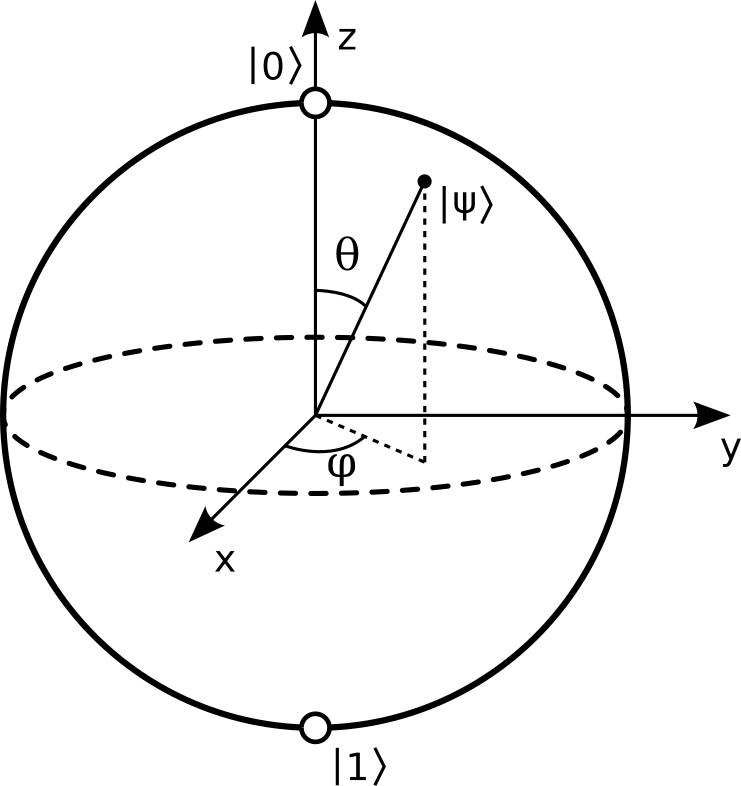
\includegraphics[width=60mm]{bloch_sphere.png}
	\caption{Bloch Sphere, courtesy of Smite-Meister on Wikipedia}
\end{figure}

In 1985, David Deutsch made headway into the theory of quantum computation. He formalized a system for general quantum computers based on the physics of the qubit. In addition, he constructed a problem that could not be easily solved by conventional computers, but could be easily solved by a quantum computer.\cite{nielsen12} The watershed moment for exploring the differences between conventional computers and quantum computers came in 1994, though, when Peter Shor showed that it was easy for a quantum computer to solve both the integer factorization problem and the discrete logarithm problem.\cite{shor95}

Unfortunately, these very problems are the problems that underpin our current public key cryptography infrastructure. RSA relies on integer factorization being a hard problem, and Diffie-Hellman and Elliptic Curve Cryptography rely on the discrete logarithm being a hard problem.\cite{kaufman02} Thus, since Shor's discovery, work has been done to find alternatives to RSA, Diffie-Hellman, and ECC cryptography. Several methods were soon recognized as being suitable replacements for our current public key systems: lattice-based methods, code-based methods, multivariate methods, and supersingular elliptic curve isogeny methods.

\section{Lattice-based Cryptography}

Consider a vector space defined by a basis $ \{ b_1, b_2, ..., b_n \} $. Then, recall that all linear combinations $ s_1 v_1 + s_2 v_2 + ... + s_n v_n $, where $ s_1, s_2, ..., s_n \in \mathbb{R} $, are in that vector space, by the definition of basis. However, given that basis, we can be more restrictive in how we use that basis. A \textit{lattice} does just that by restricting the coefficients $ s_1, s_2, ..., s_n \in \mathbb{Z} $ to be integers.\cite{bernstein09}

\begin{figure}[h!]
	\centering
	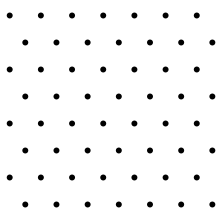
\includegraphics[width=60mm]{Equilateral_Triangle_Lattice.png}
	\caption{A lattice in $ \mathbb{R}^2 $.}
\end{figure}

When we restrict a vector space in such a way, several new, hard problems arise: the shortest vector problem (SVP), the closest vector problem (CVP), and the shortest independent vector problem (SIVP). Though all three problems are somewhat relevant for lattice-based cryptography, the SVP is the most important. Given a basis for a vector space, finding the vector on the corresponding lattice with the shortest length is a hard problem.\cite{koc15}

To illustrate how hard this problem is, the classical algorithm for finding \textit{approximate} solutions to the SVP, called the LLL algorithm, can find an approximate solution with an approximation factor of $ 2^{O(n)} $, where n is the dimensionality of the basis. Thus, approximate algorithms, though they may \textit{run} in polynomial time, can only find solutions that are exponentially away. It is conjectured that finding solutions that are within a polynomial approximation factor is impossible in polynomial time. Finding exact solutions is even worse, and the best algorithm for doing so has a $O$-category of $ 2^{O(n)} $. Most importantly, though, "there are currently no known quantum algorithms for solving lattice problems that perform significantly better than the best classical algorithms."\cite{bernstein09}

\subsection{Early Strides: Oded Goldreich, Shafi Goldwasser, and Shai Halevi}

Lattice-based cryptosystems have been explored for at least two decades. In 1997, Oded Goldreich, Shafi Goldwasser, and Shai Halevi made an early attempt at applying lattice problems to cryptography. Using the closest vector problem, they devised a one-way "trapdoor" function.\cite{goldreich97}

The GGH system:\cite{goldreich97}

\begin{itemize}
	\item Picking Keys: First, Alice picks a "good" basis $ B $ to be her private key. (A "good" basis is a basis with short, almost orthogonal vectors.) Then, Alice picks a "bad" basis $ H $, with $ L(H) = L(B) $ to be the public key.
	\item Encryption: To encrypt a message $ m $, Bob converts $ m $ to a short "noise" vector $ r $ in the vector space, picks a lattice point $ v $, and computes $ r + v $.
	\item Decryption: Alice, with her "good" basis, is able to find the the closest vector to $ r + v $, and, given that $ r $ is small enough, that closest vector will be $ v $. Finally, Alice can compute $ r + v - v $ to find $ r $, the encoded message.
\end{itemize}

Though the scheme showed some promise, its flaws were revealed two years later by Phong Nguyen at the Annual International Cryptology Conference. A major intractable flaw in the system would allow an attacker to gain some information about the plaintext. Specifically, if the attacker can gain even a small portion of the plaintext message, he or she can deduce whether a given ciphertext corresponds to the original plaintext message. In addition, given two ciphertexts, an attacker can find whether they correspond to the same plaintext message or not. In addition, he found that decrypting in the GGH scheme could be reduced to a much earlier problem. Thus, GGH is unuseable as a cryptosystem.\cite{nguyen99}

\subsection{Contemporary Lattice-based Approach: Learning with Errors}

Another lattice-based approach, learning with errors, currently shows promise. This approach in its current state is "perhaps the most efficient lattice-based cryptosystem to date supported by a theoretical proof of security." This system was proven secure against chosen plaintext attack, "based on the conjectured hardness of the learning with errors problem (LWE)." In addition, worst-case approximate-SVP and approximate-SIVP were quantum reduced to LWE, thus hinting that the LWE problem is hard.\cite{bernstein09}

The LWE problem can be described in two different ways, highlighting how LWE is related to lattices:\cite{bernstein09}

\begin{enumerate}
	\item Given $ n, m, q, a \in \mathbb{Z} $ and a probability distribution $ x $ on $ \mathbb{Z}_q $, given an arbitrary pair $(A, v)$ with $ A \in \mathbb{Z}^{m \times n}_q $ chosen uniformly, can it be deduced whether $ v $ was chosen uniformly from $ \mathbb{Z}^m_p $ or was generated from the calculation $ A s + e $ for some uniformly chosen $ s \in \mathbb{Z}^n_q $ and a vector $ e \in \mathbb{Z}^m_q $ chosen according to $ x^m $.
	\item Given a uniform $ A \in \mathbb{Z}^{m \times n}_q $ and a vector $ v \in \mathbb{Z}^m_q $, was $ v $ chosen uniformly from $ \mathbb{Z}^m_q $, or was $ v $ chosen by slightly changing a random vector in $ \Lambda_q(A^T) $ using $ x $, where $ \Lambda_q = \{ y \in \mathbb{Z}^m | y = A^Ts \mod q $ for some $ s \in \mathbb{Z}^n \}$.
\end{enumerate}

A LWE algorithm:\cite{bernstein09}

\begin{itemize}
	\item Preliminary: Define $ \Psi_\alpha $ to be a distribution of elements in $ \mathbb{Z}_q $, obtained by rounding the result of the normal distribution with mean 0 and standard deviation $ \frac {\alpha q} {\sqrt{2 \pi}} $.
	\item Preliminary: Define $ f: \mathbb{Z}^l_t \rightarrow \mathbb{Z}^l_q $ by scalar multiplying the input by $ \frac {q} {t} $, then rounding to the nearest integer.
	\item Paremeters: $ n, m, l, t, r, q \in \mathbb{Z} $ and $ \alpha \in \mathbb{R} > 0 $
	\item Private Key: Alice chooses $ S \in \mathbb{Z}^{n \times l}_q $ uniformly at random.
	\item Public key: Alice chooses $ A \in \mathbb{Z}^{m \times n}_q $ uniformly at random and $ E \in \mathbb{Z}^{m \times l}_q $ by choosing each entry according to $ \Psi $. Her public key is $ (A, P) $, where $ P = A S + E $.
	\item Encryption: Bob converts message $ m $ into $ v \in \mathbb{Z}^l_t $ and picks $ a \in \{ -r, -r + 1, ..., r - 1, r \}^m $ uniformly at random. Then, Bob computes the tuple $ (u, c) $ where $ u = A^T a $ and $ c = P^T a + f(v) $.
	\item Decryption: Alice computes $ v = f^{-1}(c - S^T u) $.
\end{itemize}

A recent incarnation of the RLWE cryptosystem was unveiled by Chris Peikert at PQCrypto 2014, where he presented a possible implementation of the scheme for use on the internet, with "drop-in replacements" for current methods of key transport, encryption, and authenticated key exchange.\cite{peikert14}

Learning with errors is perhaps the best approach for a general public key infrastructure in a post-quantum world. Although the key-space is in $ O(n^2) $, lattice-based cryptography has strong security proofs and relatively efficient implementations, making it one of the best candidates for post-quantum cryptography.\cite{bernstein09} As an added bonus, the LWE approach can be used for homomorphic encryption, as well.\cite{koc15}

\section{Code-based Cryptography}

Error correcting codes, like the ubiquitous Hamming distance-based systems, have been in use in computing applications for decades. Error correcting codes are often used in hardware applications where data integrity is paramount. ECC memory and hard drives are just two of the many applications for error correcting codes. In integrity applications, some additional bits (the code) are included with a data message to ensure that, if one or several bits of the message are flipped, the original message can still be recovered.

However, some work has been done to apply ECC to cryptography as well. The key insight for applying ECC to cryptography is that some errors can be introduced in the message to hide it (the ciphertext). Then, if only Alice has the corresponding code to correct the error, only Alice can correct the message back to its original plaintext form.\cite{bernstein09}

Robert J. McEliece was the first person to propose a code-based cryptography scheme in 1978. Thus, it is historically important to understand his scheme, as many of today's approaches are tweaks of the original formula.\cite{deneuville17}

\subsection{The McEliece Scheme}

The McEliece Algorithm:\cite{bernstein09}

\begin{itemize}
	\item Parameters: Alice picks $ n, t \in \mathbb{N} $, where $ t \ll n $.
	\item Key Generation:Alice generates the following matrices based on $ n, t $.
	\begin{itemize}
		\item $ G $: a $ k \times n $ generator matrix of a code $ g $ over $ \mathbb{F} $ of dimension $ k $ and minimum distance $ d \ge 2 t + 1 $.
		\item $ S $: a $ k \times k $ random binary non-singular matrix
		\item $ P $: a $ n \times n $ random permutation matrix 
		\item $ G_{pub} = S G P $, a $ k \times n $ matrix
	\end{itemize}
	\item Public Key: $ (G_{pub}, t) $
	\item Private Key: $ (S, D_g, P) $, where $ D_g $ is an efficient decoding algorithm for $ g $.
	\item Encryption: Bob can encrypt messages $ m \in \mathbb{F}^k $.
	\begin{enumerate}
		\item Bob chooses $ z \in \mathbb{F}^n $ of weight $ t $.
		\item Bob computes $ c = m G_{pub} \oplus z $.
	\end{enumerate}
	\item Decryption:
	\begin{enumerate}
		\item Alice computes $ c P^{-1} = (m S) G \oplus z P^{-1} $.
		\item Alice applies the decoding algorithm $ D_g $ to $ c P^{-1}$: $ D_g(c P^{-1}) = m S G $.
		\item Alice picks a set $ J \subseteq \{ 1, 2, ..., n \} $, such that the matrix constructed from the corresponding columns of $ G_{pub} $ is invertible.
		\item Alice computes $ m = (m S G)_j (G_j)^{-1} S^{-1}$.
	\end{enumerate}
\end{itemize}

Most efforts thus far have been focused on making incremental improvements to the McEliece scheme. Though the original incarnation still appears secure today, the large public keys required (ranging from 100 kilobytes to several megabytes) make the system impractical.\cite{bernstein09}\cite{deneuville17} Most efforts have been an attempt to modify the McEliece scheme to reduce the public key size. One such approach used quasi-cyclic codes as the error-correcting codes. However, this approach was vulnerable to an attack. Otmani et. Al discovered that, "a parity-check matrix of a punctured version of the secret code can be recovered in cubic time complexity in its length."\cite{otmani08}

A different, innovative approach that broke from the traditional McEliece scheme was proposed by Alekhnovich in 2003. Alekhnovich focused on deriving "a system with a security reduction to the problem of decoding random linear codes."\cite{alekhnovich03} Though the approach was innovative, the corresponding key size for Alekhnovich's system was even larger than the original McEliece system. A contemporary approach, Ouroboros, borrows from both the McEliece system and the Alekhnovich system and adapts them to key exchange, which would make it a suitable drop-in replacement for Diffie-Hellman or any other quantum-vulnerable key exchange protocols.\cite{deneuville17}

\subsection{Contemporary Approach: Ouroboros}

The Ouroboros protocol relies on decoding cyclic errors using a modified "BitFlip" algorithm. The Ouroboros Protocol:\cite{deneuville17}

\begin{itemize}
	\item Let $ w(v) $ be the hamming weight of a vector $ v $.
	\item Let $ S^n_w(\mathbb{F}_2) $ be the set of words in $ \mathbb{F}^n_2 $ of weight $ w $.
	\item Let $ f_w $ be a function which produces a vector of weight $ w $, given an entry $ r $.
	\item Let $ H: \{ 0, 1 \}* \rightarrow S^n_w(\mathbb{F}_2) $ be a hash function.
	\item Alice picks a secret, $ x, y \in S^n_w(\mathbb{F}_2) $.
	\item Alice picks a random vector $ h \in \mathbb{F}^n_2 $, then computes $ s = x + h y $, called the syndrome.
	\item Alice sends $ h, s $ to Bob.
	\item Bob picks $ r_1, r_2 \in S^n_w(\mathbb{F}_2) $
	\item Bob computes $ e_r = f_w (H(r_1, r_2)) $
	\item Bob picks a random $ \epsilon \in S^n_{w_e}(\mathbb{F}_2) $.
	\item Bob computes $ s_r = r_1 + h r_2 $, his first syndrome.
	\item Bob computes $ s_\epsilon = s r_2 + e_r + \epsilon $, his second syndrome.
	\item Bob sends $ s_r, s_\epsilon $ to Alice.
	\item Alice computes $ e_c = s_\epsilon - y s_r$.
	\item Alice uses the modified "BitFlip" algorithm to retrieve $ r_1, r_2 $ from $ x, y, e_c, t, w, w_e $.
	\item Alice computes $ \epsilon = e_c - x r_2 + y r_1 - f_w(H(r_1, r_2)) $.
	\item The shared secret is then $ \epsilon $.
\end{itemize}

The strength of the Ouroboros system is its strong passive security reductions, as it relies on Alekhnovich's construction. As Ouroboros is designed for key exchange rather than long-term public key cryptography, in general, the authors of the protocol deem the passive security reductions as sufficient, whereas long-term public key cryptography requires security reductions against active adversaries, as well.\cite{deneuville17}

As for efficiency, the public keys $ h, s \in \mathbb{F}^n_2 $, which each require $ n $ bits. The Ouroboros team illustrates the parameters required for several different bit-lengths of security:

\begin{figure}[h!]
	\centering
	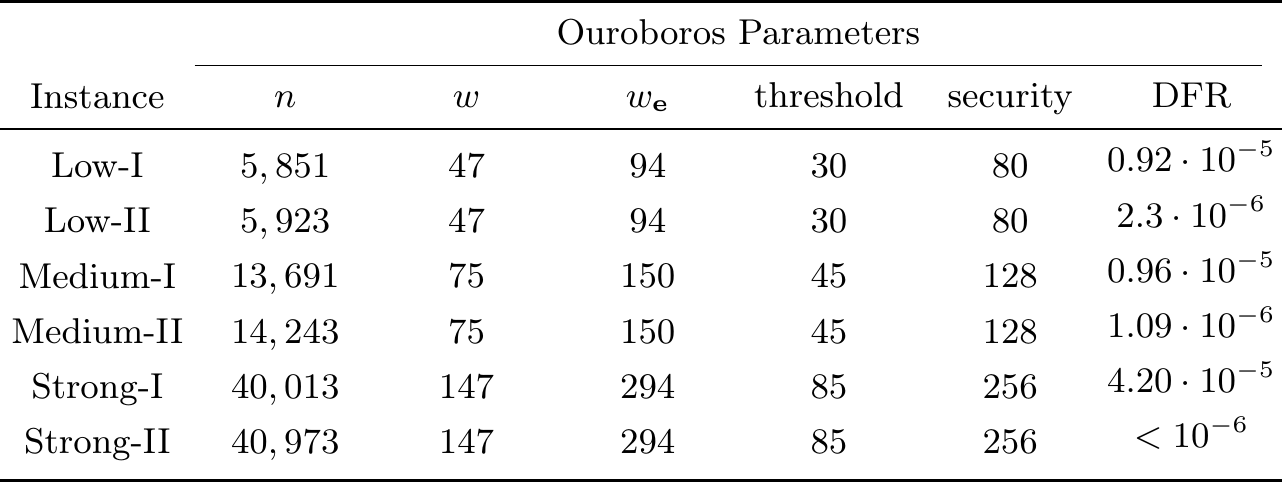
\includegraphics[width=120mm]{ouroboros_parameters.png}
	\caption{Parameters needed for corresponding bit-lengths of security\cite{deneuville17}}
\end{figure}

Thus, for 128-bit security, the public key for the Ouroboros protocol is roughly $ \ceil*{\frac {13691} {8}} \times 2 = 3424 $ bytes, or \~3.4 kilobytes, several times larger than the required key length of RSA.

Another drawback of Ouroboros is that it is a very new protocol, first unveiled at PQCrypto in 2017. More work is needed to verify its suitability as a key exchange protocol.

\section{Multivariate Cryptography}

The field of multivariate cryptography, as the name suggests, seeks to derive cryptosystems from multivariate polynomials. For example, a quadratic equation of a single variable may be $ f(x) = 14 + 2 x + x^2 $, whereas a quadratic equation of two variables may be $ f(x, y) = 6 + 2 x + 3 y + 6 x y + 4 x^2 + 2 y^2 $.

Multivariate schemes are attractive for post-quantum cryptography, as they are not affected by Shor's algorithm. In addition, they are backed by the MQ-problem, the problem of solving systems of quadratic equations over a field. This problem is NP-hard, and is thus safe from quantum attacks.\cite{cartor17eflash}

As originally conceived, multivariate systems relied on quadratic bijective functions from vector spaces into themselves. However, it was difficult to find such bijective functions with good properties. For many such bijective functions, it was either too hard or too easy to find the inverse function, and it is necessary that the function is easy to invert by holder of the private key, but hard to invert by a third party.\cite{cartor17eflash}

Alone, this is hard to accomplish, so many multivariate cryptosystems attempted to hide an easily-invertible function among two affine transformations, $ T, U $ like so: $ P = T \circ f \circ U$. In fact, the properties of these affine transformations determine the type of cryptosystem. In $ C^* $ cryptosystems, T and U are both invertible, as originally introduced in Tsutomu Matsumoto's and Hideki Imai's 1988 presentation.\cite{matsumoto88}\cite{chen15} In $ C^{*-}$ cryptosystems, T is singular, but U is invertible. In $ p C^* $ systems, U is singular, but T is invertible. Finally, in $ p C^{*-} $ systems, both T and U are singular. PFLASH is one such $ p C^{*-} $ cryptosystem.\cite{chen15}

\subsection{PFLASH}

The PFLASH algorithm was envisioned as a replacement for the previous SFLASH system, which was completely broken in 2007. Whereas SFLASH was a $ C^{*-} $ multivariate system, PFLASH sought to avoid the problems that caused SFLASH's downfall, opting to follow a $ p C^{*-} $ multivariate system, instead.\cite{chen15}

The PFLASH algorithm for signing:\cite{chen15}

\begin{itemize}
	\item Alice picks a finite field, $ \mathbb{F}_q $, with $ q $ elements.
	\item Alice picks a degree-n extension of $ \mathbb{F}_q $. Call it $ k $.
	\item There exists a vector-space isomorphism that maps $ k $ to $ \mathbb{F}^n_q $. Thus, we can treat the extension $ k $ as a vector space $ \mathbb{F}^n_q $.
	\item Define $ f: \mathbb{F}^n_q \rightarrow \mathbb{F}^n_q $ by $ f(x) = x^{q^\theta + 1} $, and ensure that $ \theta $ is chosen carefully, such that $ \gcd (q^n - 1, q^\theta + 1) = 1 $. Note that this function is easily invertible.
	\item Alice picks $ r $ and $ d $, to be used as the coranks of the matrices below.
	\item Alice picks two singular (not invertible), affine transformations $ T, U $ such that the corank of $ T $ is $ r $ and the corank of $ U $ is d. Note that since $ T, U $ are affine, they can be represented as $ T(x) = M_T x + c_T $ and $ U(x) = M_U x + c_U $, where $ M_T, M_U $ are singular.
	\item Alice hides $ f $ by calculating the public key $ P = T \circ f \circ U $.
	\item To sign a message $ m $:
	\begin{enumerate}
		\item Alice selects a preimage of $ m $ under $ T $, call it $ m^{-1}_T $.
		\item Alice inverts $ f $ and computes $ f^{-1}(m^{-1}_T) $. Call it $ m^{-1}_f $.
		\item Alice selects a preimage of $ m^{-1}_f $ under $ T $, call it $ s_m $.
	\end{enumerate}
	\item Bob verifies Alice's signature $ s_m $ by computing $ P(s_m) $, which will yield $ m $.
\end{itemize}

Ryann Cantor and Daniel Smith-Tone evaluated the security of the PFLASH system with a presentation at PQCrypto 2017. Though a recent attack had been found for $ p C^{*-} $ systems, Cantor and Smith-Tone found that PFLASH was secure against that attack. In addition, they found that "the entropy of the key space is not greatly reduced by choosing parameters that are secure against differential adversaries." Cantor and Smith-Tone concluded that "PFLASH remains a secure and attractive option for implementation in low power environments."\cite{cartor17pflash}

In addition to security, both computation and storage space are important to consider when evaluating a cryptosystem. Upon inspecting multivariate systems closer, a huge disadvantage becomes obvious. Public keys for the system are huge. For example, for 80 bits of security, the corresponding PFLASH public key must be 39,040 bytes. For 128 bit security, this number grows to 142,848 bytes.\cite{chen15} However, an equally important advantage of the system is that it requires far fewer computations than either elliptic curve cryptography or RSA. In the context of embedded systems, this is very important,\cite{bernstein09} and, indeed PFASH is a system designed to be suitable for producing signatures on smart cards. While there is a trade-off between computation speed and storage, multivariate systems like PFLASH may be perfect for securing smart cards against quantum computers.

\section{Conclusion}

Three post-quantum approaches show promise at replacing the currently broken public key systems of RSA, Diffie-Hellman, and elliptic curve cryptography: Lattice-based approaches, code-based approaches, and multivariate approaches.

Learning with errors, a lattice-based approache, is perhaps the best approach for a general public key infrastructure in a post-quantum world. Although the key-space is in $ O(n^2) $, lattice-based cryptography has strong security proofs and relatively efficient implementations, making it one of the best candidates for post-quantum cryptography.\cite{bernstein09} As an added bonus, the LWE approach can be used for homomorphic encryption, as well.\cite{koc15}

Though code-based cryptography is promising, it had not received much attention before post-quantum cryptography become a major field of research. One potential reason for that is that, simply, RSA, Diffie-Hellman, and elliptic curve cryptography have been sufficient solutions thus far, and so there was no pressing reason to research an alternative.\cite{bernstein09} Perhaps the most convincing reasons, though, are code-based cryptography's major drawbacks. First, the system can be reduced to "an ad-hoc problem, the difficulty of recovering the hidden structure of a decodable code from a public matrix." Second, as mentioned earlier, public key sizes are very large.\cite{deneuville17} They can range from 100 kilobytes to several megabytes.\cite{bernstein09} However, Ouroboros cuts this key size down to several kilobytes for key exchange. In addition, Ouroboros has strong passive security reductions. However, Ouroboros is still very new, and thus should not be considered a suitable replacement until it has reached maturity and found to be safe to use.

Lastly, multivariate cryptography shows promise in low-power signing applications, like smart cards. PFLASH was shown to be secure at PQCrypto 2017. As flash memory and ROM prices decrease, the required storage for the PFLASH system may become less of a hindrance. In addition, it requires far fewer computations than either elliptic curve cryptography or RSA. In the context of embedded systems, this is very important,\cite{bernstein09} and, indeed PFASH is a system designed to be suitable for producing signatures on smart cards. While there is a trade-off between computation speed and storage, multivariate systems like PFLASH may be perfect for securing smart cards against quantum computers.

\begin{thebibliography}{99}

\bibitem{kaufman02}
	Charlie Kaufman, Radia Perlman, Mike Speciner.
	\textit{Network Security: Private Communication in a Public World},
	2nd ed.
	Prentice Hall,
	Upper Saddle River, New Jersey,
	2002.
	
\bibitem{nielsen12}
	Michael Nielsen, Isaac Chuang.
	\textit{Quantum Computation and Quantum Information},
	10th anniv. int'l ed.
	Cambridge University Press,
	2012.
	
\bibitem{bernstein09}
	Daniel Bernstein, Johannes Buchmann, Erik Dahmén.
	\textit{Post-quantum Cryptography}.
	Springer,
	Berlin,
	2009.
	
\bibitem{koc15}
	\c Cetin Kaya Ko\c c.
	\textit{Open Problems in Mathematics and Computational Science}.
	Springer International Publishing,
	Cham,
	2015.
	
\bibitem{shor95}
	Peter Shor.
	"Polynomial-Time Algorithms for Prime Factorization and Discrete Logarithms on a Quantum Computer."
	Cornell University Library,
	1995.
	https://arxiv.org/abs/quant-ph/9508027
	
\bibitem{nistcsrc16}
	Cryptographic Technology Group.
	"Submission Requirements and Evaluation Criteria for the Post-Quantum Cryptography Standardization Process."
	NIST CSRC,
	2016.
	http://csrc.nist.gov/groups/ST/post-quantum-crypto/documents/call-for-proposals-final-dec-2016.pdf
	
\bibitem{goldreich97}
	Oded Goldreich, Shafi Goldwasser, Shai Halevi.
	"Public-key Cryptosystems from Lattice Reduction Problems."
	1997.
	https://groups.csail.mit.edu/cis/pubs/shafi/1997-lncs-ggh.pdf
	
\bibitem{nguyen99}
	Phong Nguyen.
	"Cryptanalysis of the Goldreich-Goldwasser-Halevi Cryptosystem from Crypto ’97."
	1999.
	https://link.springer.com/content/pdf/10.1007%2F3-540-48405-1_18.pdf
	
\bibitem{peikert14}
	Chris Peikert.
	"Lattice Cryptography for the Internet."
	PQCrypto 2014: International Workshop on Post-Quantum Cryptography,
	2014.
	https://web.eecs.umich.edu/~cpeikert/pubs/suite.pdf
	
\bibitem{otmani08}
	Ayoub Otmani, Jean-Pierre Tillich, Leonard Dallot.
	"Cryptanalysis of Two McEliece Cryptosystems Based on Quasi-Cyclic Codes."
	Cornell University Library,
	2008.
	https://arxiv.org/abs/0804.0409
	
\bibitem{alekhnovich03}
	Michael Alekhnovich.
	"More on Average Case vs Approximation Complexity."
	44th Symposium on Foundations of Computer Science,
	2003.
	http://www.cs.toronto.edu/~toni/Courses/PCP/handouts/misha.pdf
	
\bibitem{deneuville17}
	Jean-Christophe Deneuville, Philippe Gaborit, Gilles Z\'emor.
	"Ouroboros: A Simple, Secure and Efficient Key Exchange Protocol Based on Coding Theory."
	PQCrypto 2017: International Workshop on Post-Quantum Cryptography,
	2017.
	https://www.researchgate.net/publication/318145380\_Ouroboros\_A\_Simple\_Secure\_and\_Efficient\_Key\_
	Exchange\_Protocol\_Based\_on\_Coding\_Theory
	
\bibitem{matsumoto88}
	Tsutomu Matsumoto, Hideki Imai.
	"Public Quadratic Polynomial-Tuples for Efficient Signature-Verification and Message-Encryption."
	Eurocrypt '88,
	1988.
	https://link.springer.com/content/pdf/10.1007\%2F3-540-45961-8\_39.pdf
	
\bibitem{chen15}
	Ming-Shing Chen, Bo-Yin Yang, Daniel Smith-Tone.
	"PFLASH - Secure Asymmetric Signatures on Smart Cards."
	2015.
	https://csrc.nist.gov/csrc/media/events/lightweight-cryptography-workshop-2015/documents/papers/session3-smith-tone-paper.pdf
	
\bibitem{cartor17pflash}
	Ryann Cartor, Daniel Smith-Tone.
	"An Updated Security Analysis of PFLASH."
	PQCrypto 2017: International Workshop on Post-Quantum Cryptography,
	2017.
	https://link.springer.com/chapter/10.1007%2F978-3-319-59879-6_14
	
\bibitem{cartor17eflash}
	Ryann Cartor, Daniel Smith-Tone.
	"EFLASH: A New Multivariate Encryption Scheme."
	2017.
	https://eprint.iacr.org/2017/1184.pdf

\end{thebibliography}

\end{document}